\documentclass[twoside]{article}

%\usepackage{aistats2021}
% If your paper is accepted, change the options for the package
% aistats2021 as follows:
%
\usepackage[accepted]{aistats2022}
%
% This option will print headings for the title of your paper and
% headings for the authors names, plus a copyright note at the end of
% the first column of the first page.

% If you set papersize explicitly, activate the following three lines:
%\special{papersize = 8.5in, 11in}
%\setlength{\pdfpageheight}{11in}
%\setlength{\pdfpagewidth}{8.5in}

% If you use natbib package, activate the following three lines:
\usepackage[round]{natbib}
\renewcommand{\bibname}{References}
\renewcommand{\bibsection}{\subsubsection*{\bibname}}

% If you use BibTeX in apalike style, activate the following line:
%\bibliographystyle{apalike}

\usepackage[colorlinks=true,linkcolor=blue,citecolor=blue]{hyperref}

\usepackage{acronym}
\usepackage{amsfonts}
\usepackage{amsfonts}
\usepackage{amsmath}
\usepackage{amssymb}
\usepackage{amsthm}
\usepackage{bbold}
\usepackage{booktabs}
\usepackage{color}
\usepackage{graphics}
\usepackage{microtype}
\usepackage{nicefrac}
\usepackage{caption}
\usepackage{float}
\usepackage{tcolorbox}

\newtcolorbox{custombox}[1][]
{
  colframe=blue!40,
  colback=blue!8,
  left=2pt,
  right=2pt,
  top=2pt,
  bottom=2pt,
  #1
}

% Custom definitions
\newtheorem{lemma}{Lemma}
\newtheorem{theorem}{Theorem}
\newtheorem{corollary}{Corollary}
\newtheorem{definition}{Definition}
\DeclareMathOperator*{\argmax}{arg\,max}
\DeclareMathOperator*{\argmin}{arg\,min}
\DeclareMathOperator{\logit}{\sigma^{-1}}
\DeclareMathOperator{\sigmoid}{\sigma}
\DeclareMathOperator{\vtheta}{\boldsymbol\vartheta}
\DeclareMathOperator{\vx}{\boldsymbol x}
\renewcommand*{\d}[1]{\operatorname{d}\!{#1}}

\newcommand{\code}[1]{\href{#1}{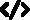
\includegraphics[scale=0.8,trim=0 0.05cm 0 0]{figures/code}}}

\newcommand{\nre}{\textsc{nre}}
\newcommand{\snre}{\textsc{snre}}
\newcommand{\npe}{\textsc{npe}}
\newcommand{\snpe}{\textsc{snpe}}
\newcommand{\kl}{\textsc{kl}}
\newcommand{\nf}{\textsc{nf}}

\begin{document}

% If your paper is accepted and the title of your paper is very long,
% the style will print as headings an error message. Use the following
% command to supply a shorter title of your paper so that it can be
% used as headings.
%
\runningtitle{Towards Drawing Scientific Conclusions with Simulation-Based Inference}

% If your paper is accepted and the number of authors is large, the
% style will print as headings an error message. Use the following
% command to supply a shorter version of the authors names so that
% they can be used as headings (for example, use only the surnames)
%
\runningauthor{Hermans, Delaunoy, Rozet, Wehenkel, Louppe}

\twocolumn[

\aistatstitle{Averting A Crisis In Simulation-Based Inference}

\aistatsauthor{%
  Joeri Hermans*\\
  %Montefiore Institute\\
  University of Li{\`e}ge\\
  \texttt{joeri.hermans@doct.uliege.be} \\
  % examples of more authors
  \And
  Arnaud Delaunoy*\\
  %Montefiore Institute\\
  University of Li{\`e}ge\\
  \texttt{a.delaunoy@uliege.be} \\
  \AND
  François Rozet \\
  University of Li{\`e}ge\\
  \texttt{francois.rozet@uliege.be} \\
  \And
  Antoine Wehenkel \\
  %Montefiore Institute\\
  University of Li{\`e}ge\\
  \texttt{a.wehenkel@uliege.be} \\
  \And
  Gilles Louppe \\
  %Montefiore Institute\\
  University of Li{\`e}ge\\
  \texttt{g.louppe@uliege.be} \\
}

\aistatsaddress{%
}]

\begin{abstract}
We present extensive empirical evidence showing that current Bayesian simulation-based inference algorithms are inadequate for the falsificationist methodology of scientific inquiry.
Our results collected through massive experimental computations show that all benchmarked algorithms -- \textsc{(s)npe}, \textsc{(s)nre}, \textsc{snl} and variants of \textsc{abc} -- may produce overconfident posterior approximations, which makes them demonstrably unreliable and dangerous if one's scientific goal is to constrain parameters of interest. %, as is often the case in the physical sciences.
We believe that failing to address this issue will lead to a well-founded trust crisis in simulation-based inference.
For this reason, we argue that research efforts should now focus on theoretical and methodological developments of conservative approximate inference algorithms and present research directions towards this objective.
In this regard, we show empirical evidence that ensembles are consistently more reliable.

\end{abstract}

\section{Introduction}

Many scientific disciplines rely on computer simulations to study complex phenomena under various conditions.
Although modern simulators can generate realistic synthetic observables through detailed descriptions of their data generating processes, they are unfortunately not suitable for statistical inference.
The computer code describing the data generating processes defines the likelihood function $p(\vx\vert\vtheta)$ only implicitly, and its direct evaluation requires the often \emph{intractable} integration of all stochastic execution paths.
In this problem setting, statistical inference based on the likelihood function becomes impractical, but approximate inference remains possible by relying on likelihood-free \emph{approximations}, as pushed forward by the rapidly expanding field of simulation-based inference \citep{cranmer2020frontier}.

While simulation-based inference targets domain sciences, advances in the field are mainly driven from a machine learning perspective.
The field, therefore, inherits the quality assessments \citep{lueckmann2021benchmarking} customary to the machine learning literature, such as the minimization of classical divergence criteria.
Despite recent developments of post hoc diagnostics to inspect the quality of likelihood-free approximations \citep{cranmer2015approximating, Brehmer:2018eca, brehmer2019mining, Hermans:2020skz, lueckmann2021benchmarking, sbc, dalmasso2020confidence}, assessing whether approximate inference results are sufficiently reliable for scientific inquiry remains largely unanswered whenever fitting criteria are not globally optimized or whenever the data is limited.
In fact, domain sciences, and more specifically the physical sciences, are not necessarily interested in \emph{accuracy} or \emph{correctness} of an approximation.
Instead, in the tradition of Popperian falsification, they often seek to {\bfseries constrain parameters} of interest as much as possible at a given confidence level.
Scientific examples include frequentist confidence intervals on the mass of the Higgs boson \citep{aad2012observation}, Bayesian credible regions on cosmological parameters \citep{gilman2018probing,Planck:2018vyg}, or constraints on the intrinsic parameters of binary black hole coalescences \citep{abbott2016gw151226}.
From a Bayesian perspective, this implies that statistical approximations in simulation-based inference should ideally come with \emph{conservative} guarantees to not produce credible regions smaller than they should be, even if it incurs a loss in statistical power.
Wrongly constraining model parameters would otherwise impede scientific inquiry.

In this work, we measure the quality of the credible regions computed through various Bayesian techniques in simulation-based inference and do so through the notion of \emph{coverage}.
We frame our main contribution as the collection of extensive empirical evidence that required months of computation.
Our results demonstrate that all benchmarked techniques can produce non-conservative credible regions, highlighting the need for a new class of conservative approximate inference algorithms.
The structure of the paper is outlined as follows.
Section \ref{sec:background} describes the statistical formalism, necessary background and includes a thorough motivation for coverage.
Section \ref{sec:experiments} highlights our main results.
Section \ref{sec:discussion} presents several avenues of future research to {\bfseries enable drawing reliable scientific conclusions} with simulation-based inference. All code related to this manuscript is available at
\href{https://github.com/montefiore-ai/crisis-in-sbi}{\texttt{github.com/montefiore-ai/crisis-in-sbi}}
\section{Background}
\label{sec:background}

\subsection{Statistical formalism}
\label{sec:statistical_formalism}
We evaluate posterior estimators that produce approximations $\hat{p}(\vtheta\vert\vx)$ with the following semantics.

{\bf Target parameters} $\vtheta$ denote the parameters of interest of a simulation model, and are sometimes referred to as \emph{free} or \emph{model} parameters. The precise definition of $\vtheta$ depends on the problem setting. We make the reasonable assumption that the prior $p(\vtheta)$ is a known and tractable quantity.

The {\bf observable} $\vx$ denotes the synthetic realizations of the simulator. Observed data $\vx_o$ is the observable we would like to do inference on, under the assumption that the simulation model is correctly specified.

The {\bf likelihood} model $p(\vx\vert\vtheta)$ implicitly defined by the simulator's computer code. While we cannot evaluate the density $p(\vx\vert\vtheta)$, we \emph{can} simulate samples.

The {\bf ground truth} $\vtheta^*$ specified to the simulation model whose forward evaluation produced the observable $\vx_o$, i.e., $\vx_o\sim p(\vx\vert\vtheta=\vtheta^*)$.

The {\bf credible region} is a space $\Theta$ within the target parameter domain that satisfies
\begin{equation}
    \int_\Theta p(\vtheta\vert\vx=\vx_o) \d{\vtheta} = 1 - \alpha
\end{equation}
for some observable $\vx_o$ and confidence coefficient $1 - \alpha$.
Because many such regions exist, we compute the credible region with the \emph{smallest} volume. In the literature this credible region is known as
the \emph{highest posterior density region} \citep{box2011bayesian,hyndman1996computing}.

\subsection{Statistical quality assessment}
\begin{figure}[b!]
    \centering
    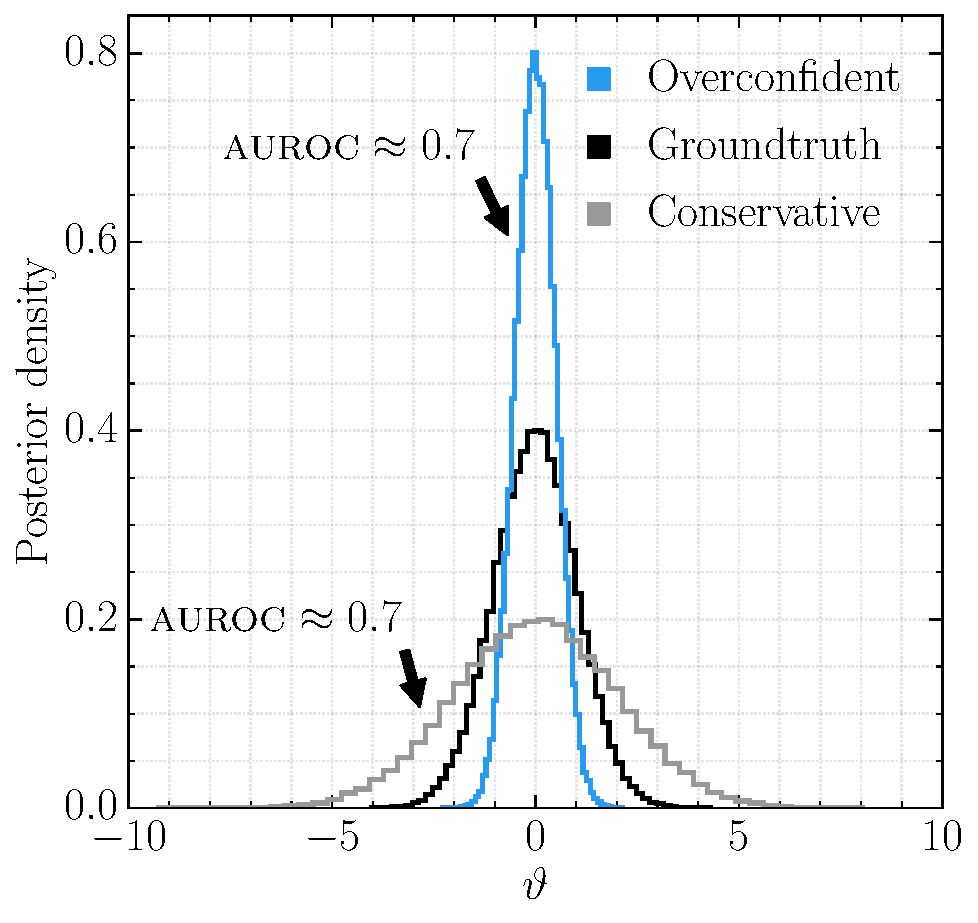
\includegraphics[width=\linewidth]{figures/auc-deceitful.pdf}
    \caption{A classifier-based metric measures the divergence between posterior approximations and a ground truth by means of evaluating the classifier's discriminative performance through Area Under the Receiver Operating Characteristics curve (\textsc{auroc}). In this case, the metric argues that both the conservative and overconfident approximations are equally accurate since the metric yields \textsc{auroc} = 0.7 for both approximations. From an inference perspective however, the conservative approximation is clearly more suitable because it produces credible regions larger than they should be.}
    \label{fig:auc_deceitful}
\end{figure}
The main problem with metrics such as the Classifier Two-sample Test \citep{lehmann2006testing,lopez2016revisiting} or Maximum Mean Discrepancy \citep{gretton2012kernel,bengio2013bounding,dziugaite2015training} is that they assess \emph{accuracy} or \emph{closeness} of an approximation through a divergence with respect to a posterior that is intractable in practice.
Even if such evaluations would hypothetically be possible,
there are no criteria to what constitutes an \emph{acceptable}
In addition, it is not possible to know for certain whether the classifier or kernel used to measure the diverge are sufficiently expressive to detect differences between the approximation and said posterior.

To clarify these points, consider the demonstration in Figure \ref{fig:auc_deceitful}.
A binary classifier is trained to discriminate between samples from a posterior approximation and the true posterior.
The discriminative performance of the classifier is expressed through Area Under the Receiver Operating Characteristics curve (\textsc{auroc}) and serves as a measure for divergence between both densities. An \textsc{auroc} = 0.5 suggests an approximation that is indistinguishable from the true posterior, while \textsc{auroc} = 1.0 implies that both densities do not overlap.
Although both approximations in our demonstration are equally accurate according to the \textsc{auroc}, the \emph{overconfident} approximation demonstrates the potential trust crisis in simulation-based inference:
producing credible regions that are biased or smaller than they should be, leading to erroneous scientific conclusions.
For this reason, we take the position that posterior approximations should, irrespective of the available simulation budget, produce inflated credible regions and do not have to closely match the true posterior to draw meaningful inferences.

Instead of measuring accuracy of approximations with respect to an intractable posterior, this work directly probes
the quality of credible regions through \emph{coverage}: a quantity that can be estimated in practice and has a criterion to determine acceptable approximations.
\begin{definition}
The {\bfseries coverage probability} of a posterior estimator at a confidence coefficient $1 - \alpha$ is
\begin{equation}
    \int_{\vtheta}\int_{\vx} p(\vtheta,\vx)~\mathbb{1}\left[\vtheta \in \Theta_{\hat{p}(\vtheta|\vx = \vx)}(1 - \alpha)\right]~\d\vtheta\d\vx,
\end{equation}
where the function
$\Theta_{p(\vtheta\vert\vx)}(1 - \alpha)$ yields the $1 - \alpha$ highest posterior density region
of $\hat{p}(\vtheta\vert\vx)$.
\end{definition}
\begin{definition}
The {\bfseries empirical coverage probability} of a posterior estimator at a confidence coefficient $1 - \alpha$ given a set of $n$ i.i.d. samples $(\vtheta^*,\vx)\sim p(\vtheta,\vx)$
is
\begin{equation}
\frac{1}{n} \sum_{i=1}^n ~\mathbb{1}\left[\vtheta^*_i \in \Theta_{\hat{p}(\vtheta|\vx = \vx_i)}(1 - \alpha)\right].
\end{equation}
\end{definition}
\begin{definition}
The {\bfseries nominal coverage probability} is the coverage probability of the true posterior and is equal to the known confidence level $(1 - \alpha)\cdot 100\%$.
\end{definition}
\begin{definition}
A posterior estimator is deemed acceptable if it {\bfseries has coverage} at the confidence level of interest, i.e., whenever the empirical coverage probability is {\bfseries larger or equal} to the nominal coverage probability.
\end{definition}
\begin{definition}
A {\bfseries conservative estimator} is an estimator that has coverage for {\bfseries all} confidence levels.
\end{definition}
Although coverage is a necessary metric to assess conservativeness, it is limited in its ability to determine the information gain a posterior (approximation) has over its prior. To clarify this point, consider an estimator whose posteriors are identical to the prior. In this case, there is no gain in information and the empirical coverage probability is equal to the nominal coverage probability. For this reason, a complete analysis should be complemented with measures such as the mutual information or expected information gain $\mathbb{E}_{p(\vtheta,\vx)}\left[\log p(\vtheta\vert\vx) - \log p(\vtheta)\right]$.
This work however is concerned with {\bfseries conservative inference} and will therefore limit the analysis to the evaluation of coverage. Finally, it should be noted that coverage is a statement about the credible regions in expectation. Coverage does not make any statement about the quality of a single posterior.

\section{Experimental observations}
\label{sec:experiments}
This section covers our main contribution: the collection of empirical evidence to determine whether approaches in simulation-based inference are conservative by nature.
We are particularly interested in determining \emph{if} certain approaches should be
favoured over others. We do so by measuring the coverage of estimators attained by these approaches across a broad range of hyperparameters and benchmarks of varied complexity, including two \emph{real} problems from the field of astronomy.
As in real use-cases, the true posteriors associated with these benchmarks are unknown.
Hyperparameters are listed in Appendix \ref{appendix:hyperparameters}.
\subsection{Methods}
\label{sec:methods}
We make the distinction between two paradigms.
Non-amortized approaches are designed to approximate a \emph{single} posterior, while amortized methods aim to learn a general purpose estimator that attempts to approximate \emph{all} posteriors supported by the prior.
\subsubsection{Amortized}
{\bf Neural Posterior Estimation} (\npe) is concerned with directly learning an amortized estimator $\hat{p}_\psi(\vtheta\vert \vx)$ to the posterior with normalizing flows. Normalizing flows define a class of probability distributions $p_\psi(\cdot)$ built from neural network based bijective transformations \citep{dinh2014nice,dinh2016density} parameterized by $\psi$ and are usually optimized via
$\argmin_\psi \mathbb{E}_{p(\vx)} \left[\textsc{kl}(p(\vtheta|\vx)~\vert\vert ~\hat{p}_\psi(\vtheta|\vx)\right]$,
which is equivalent to $\argmax_\psi \mathbb{E}_{p(\vtheta,\vx)}\left[\log \hat{p}_\psi(\vtheta|\vx)\right]$.
Once trained, the density of the modeled distribution can easily be evaluated \emph{and} sampled from.

{\bf Neural Ratio Estimation} (\nre) is an established approach in the simulation-based inference literature both from a frequentist \citep{cranmer2015approximating} and Bayesian \citep{thomas2016likelihood,2019arXiv190304057H} perspective. In a Bayesian analysis,
an amortized estimator $\hat{r}(\vx\vert\vtheta)$
of the \emph{intractable} likelihood-to-evidence ratio $r(\vx\vert\vtheta)$ can be learned by training a binary discriminator $\hat{d}(\vtheta,\vx)$ with inputs $\vtheta$ and $\vx$ to distinguish between samples of the
joint $p(\vtheta,\vx)$ with class label 1 and samples of the product of marginals $p(\vtheta)p(\vx)$ with class label 0 using a criterion such
as the binary cross entropy. Similar to the density-ratio trick \citep{sugiyama2012density,goodfellow2014generative,cranmer2015approximating,2019arXiv190304057H}, the Bayes optimal discriminator $d(\vtheta,\vx)$ models
\begin{align}
  \frac{p(\vtheta, \vx)}{p(\vtheta,\vx) + p(\vtheta)p(\vx)} = \sigmoid\left(\log\frac{p(\vtheta,\vx)}{p(\vtheta)p(\vx)}\right),
\end{align}
where $\sigmoid(\cdot)$ is the sigmoid function.
Given a target parameter $\vtheta$ and observable $\vx$ supported by $p(\vtheta)$ and $p(\vx)$ respectively,
the learned discriminator $\hat{d}(\vtheta,\vx)$ approximates the log likelihood-to-evidence ratio $\log r(\vx\vert\vtheta)$ through the logit function $\logit(\cdot)$ because
\begin{align}
  \log \hat{r}(\vx\vert\vtheta) &= \logit\left(\hat{d}(\vtheta,\vx)\right) = \log\frac{\hat{d}(\vtheta,\vx)}{1 - \hat{d}(\vtheta,\vx)}\\
  &\approx \log\frac{p(\vtheta, \vx)}{p(\vtheta)p(\vx)} = \log\frac{p(\vx\vert\vtheta)}{p(\vx)}.
\end{align}
The log posterior density function is approximated as $\log \hat{p}(\vtheta\vert\vx) = \log p(\vtheta) + \log \hat{r}(\vx\vert\vtheta)$.

{\bf Ensembles} An ensemble model \emph{averages} the approximated posteriors of $n$ separately trained posterior estimators. While this formulation is natural for \textsc{npe}, averaging likelihood-to-evidence ratios is equivalent, because
\begin{equation}
    \frac{p(\vtheta)}{n} \sum_{i=1}^n \hat{r}_i(\vx \vert \vtheta) = \frac{1}{n}\sum_{i=1}^n \hat{p}_i(\vtheta \vert \vx).
\end{equation}
\subsubsection{Non-amortized}
Rejection {\bf Approximate Bayesian Computation} \textsc{(abc)} \citep{rubin1984,pritchard1999population}
numerically estimates a \emph{single} posterior by collecting samples $\vtheta\sim p(\vtheta)$ whenever
$\vx\sim p(\vx\vert\vtheta)$ is \emph{similar} to $\vx_o$. Similarity is expressed by means of a \emph{distance function} $\rho$. For high-dimensional observables, the probability of simulating an observable $\vx$ such that $\vx = \vx_o$ is extremely small. For this reason, \textsc{abc} uses a \emph{summary statistic} $s$ and an \emph{acceptance threshold} $\epsilon$. Using these components, \textsc{abc} accepts samples into the approximate posterior whenever $\rho(s(\vx),s(\vx_o))\leq\epsilon$. In our experiments we use the identity function as a sufficient summary statistic. Finally, we emphasize that
\textsc{abc} approximations are \emph{only exact} whenever the summary statistic is sufficient \emph{and} the acceptance threshold $\epsilon$ tends to 0 \citep{sisson2018overview}.

Sequential methods aim to approximate a single posterior by \emph{iteratively} improving a posterior approximation. These methods alternate between a simulation and exploitation phase. The latter being designed to take \emph{current} knowledge into account such that subsequent simulations can be focused on parameters that are more likely to produce observables $x$ similar to $x_o$.

{\bfseries Sequential Monte-Carlo ABC} (\textsc{smc-abc}) \citep{10.1093/bioinformatics/btp619, sisson2007sequential, beaumont2009adaptive}
iteratively updates a set of proposal states to match the posterior distribution. At each iteration, accepted proposals are ranked by distance. The rankings determine whether a proposal is propagated to the next iteration. New candidate proposals are generated by perturbing the selected ranked proposals.

{\bfseries Sequential Neural Posterior Estimation} (\snpe) \citep{papamakarios2016fast, lueckmann2017flexible, greenberg2019automatic} directly models the posterior.
Our evaluations will specifically use the \textsc{snpe-c} \citep{greenberg2019automatic} variant.

{\bfseries Sequential Neural Likelihood} (\textsc{snl}) \citep{papamakarios2019sequential} models the likelihood $p(\vx|\vtheta)$. A numerical approximation of the posterior is obtained by plugging the learned likelihood estimator into a Markov Chain Monte Carlo (\textsc{mcmc}) sampler as a surrogate likelihood.

{\bfseries Sequential Neural Ratio Estimator} (\snre) \citep{2019arXiv190304057H,durkan2020contrastive} iteratively improves the modelled likelihood-to-evidence ratio.
\subsection{Benchmarks}
Our evaluations consider 7 benchmarks, ranging from toy problems to real applications in astronomy. Appendix \ref{appendix:simulation_times} lists the expected wall-clock time to generate 1000 simulations on a single CPU core.

The \emph{SLCP} simulator models a fictive problem with 5 parameters. The observable $\vx$ is composed of 8 scalars which represent the 2D-coordinates of 4 points.
The coordinate of every point is sampled from the same multivariate Gaussian whose mean and covariance matrix are the parameters $\vtheta$. We consider a simplified version of the original task \citep{papamakarios2019sequential} by inferring the marginal posterior density of 2 of those parameters. In contrast to its original formulation, the likelihood is not tractable due to the marginalization.

The \emph{Weinberg} problem \citep{weinberg} concerns a simulation of high energy particle collisions $e^+e^- \to \mu^+ \mu^-$. The angular distributions of the particles can be used to measure the Weinberg angle $\vx$
in the standard model of particle physics. From the scattering angle, we are interested in inferring Fermi's constant $\vtheta$.

The \emph{Spatial SIR} model generates a grid-world $\vx$ of susceptible,
infected, and recovered individuals. This information is encoded in 3
channels. Based on the initial state of $\vx$ and the infection and recovery rate $\vtheta$,
the model describes the evolution of an infection through this grid-like world.
The disease spreads spatially.

Originally introduced by \citet{papamakarios2019sequential}, \emph{M/G/1} models a processing and arrival queue. The problem is
described by 3 parameters $\vtheta$ that influence the time it takes to serve a customer, and the time between their arrivals. The observable $\vx$ is composed of 5 equally spaced quantiles of inter-departure times.

The \emph{Lotka-Volterra} population model \citep{lotka,volterra1926fluctuations} describes a process of interactions between a predator and a prey species. The model is conditioned by 4 parameters $\vtheta$ which influence the reproduction and mortality rate of the predator and prey species. We infer the marginal posterior of the 2 predator's parameters. Our implementation, described by a Markov process, generates 2 time-series of 1001 samples representing the evolution of the prey and predator populations over time.

Stellar \emph{Streams} form due to the disruption of spherically packed clusters of stars by the Milky Way. Because of their distance from the galactic center and other visible matter, \emph{distant} stellar streams are considered to be ideal probes to detect gravitational interactions with dark matter. The simulation model \citep{bovy2015galpy,banik2018probing,Hermans:2020skz} evolves the stellar density $\vx$ of a stream over several billion years, while perturbing the stream over its evolution through interactions with dark matter subhaloes parameterized through the dark matter particle mass $\vtheta$.

\emph{Gravitational Waves (GW)} are ripples in space-time emitted during events such as the collision of two black-holes. They can be detected through interferometry $\vx$ and convey information about the celestial bodies, unlocking a new way to study the universe. We consider the task of inferring the masses $\vtheta$ of two black-holes colliding through the observation of the gravitational wave as measured by \textsc{ligo}'s dual detectors \citep{lalsuite,Biwer:2018osg}.

\subsection{Setup}
Our evaluations consider simulation budgets ranging from $2^{10}$ up to $2^{17}$ samples and confidence levels from 0.05 up to 0.95. Within the \emph{amortized} setting
we train, for every simulation budget, 5 posterior estimators for 100 epochs. The empirical coverage probability is
computed on at least 5,000 unseen samples from the joint $p(\vtheta,\vx)$ and for all confidence levels under consideration.
In addition, we repeat the coverage evaluation for ensembles of 5 estimators as well.

Special care for \emph{non-amortized} approaches is necessary because they only approximate a \emph{single} posterior and can therefore not evaluate coverage.
Our experiments estimate coverage of these methods \emph{by proxy} by repeating the inference procedure on 300 distinct observables for a given simulation budget (2100 times per method per benchmark).
The empirical coverage probabilities are subsequently estimated using the 300 approximated posteriors.
Our experiments with \textsc{npe}, \textsc{snpe}, \textsc{snl}, \textsc{snre}, \textsc{rej-abc} and \textsc{smc-abc} rely on \texttt{sbi}'s \citep{sbi} reference implementation, while we use a custom implementation for \textsc{nre}.

{\bfseries Computational cost} We would like to emphasize the computational requirements necessary to generate our main contribution: the experimental observations, whose generation took months on several computer clusters. The bulk of the cost was associated with the repeated optimization procedure of non-amortized methods and the constant resampling of the simulator.

\subsection{Results}
\protect\begin{custombox}
{\bfseries Observation 1} All benchmarked algorithms produce non-conservative posterior approximations. This pathology tends to be accentuated when using a small simulation-budget in both amortized and non-amortized approaches.

\medskip

{\bfseries Observation 2} For a given simulation budget, amortized approaches have the tendency to be more conservative than non-amortized approaches.

\medskip

{\bfseries Observation 3} The empirical coverage probability of an ensemble model is larger than the expected individual model. The ensemble size positively affects the empirical coverage probability as well.

\medskip

{\bfseries Observation 4} Amortized methods are not subordinate with respect to the simulation-efficiency of non-amortized sequential methods, especially when taking hyper-parameter tuning and the evaluation of the coverage diagnostic into account.
\end{custombox}
\begin{figure*}[h!]
    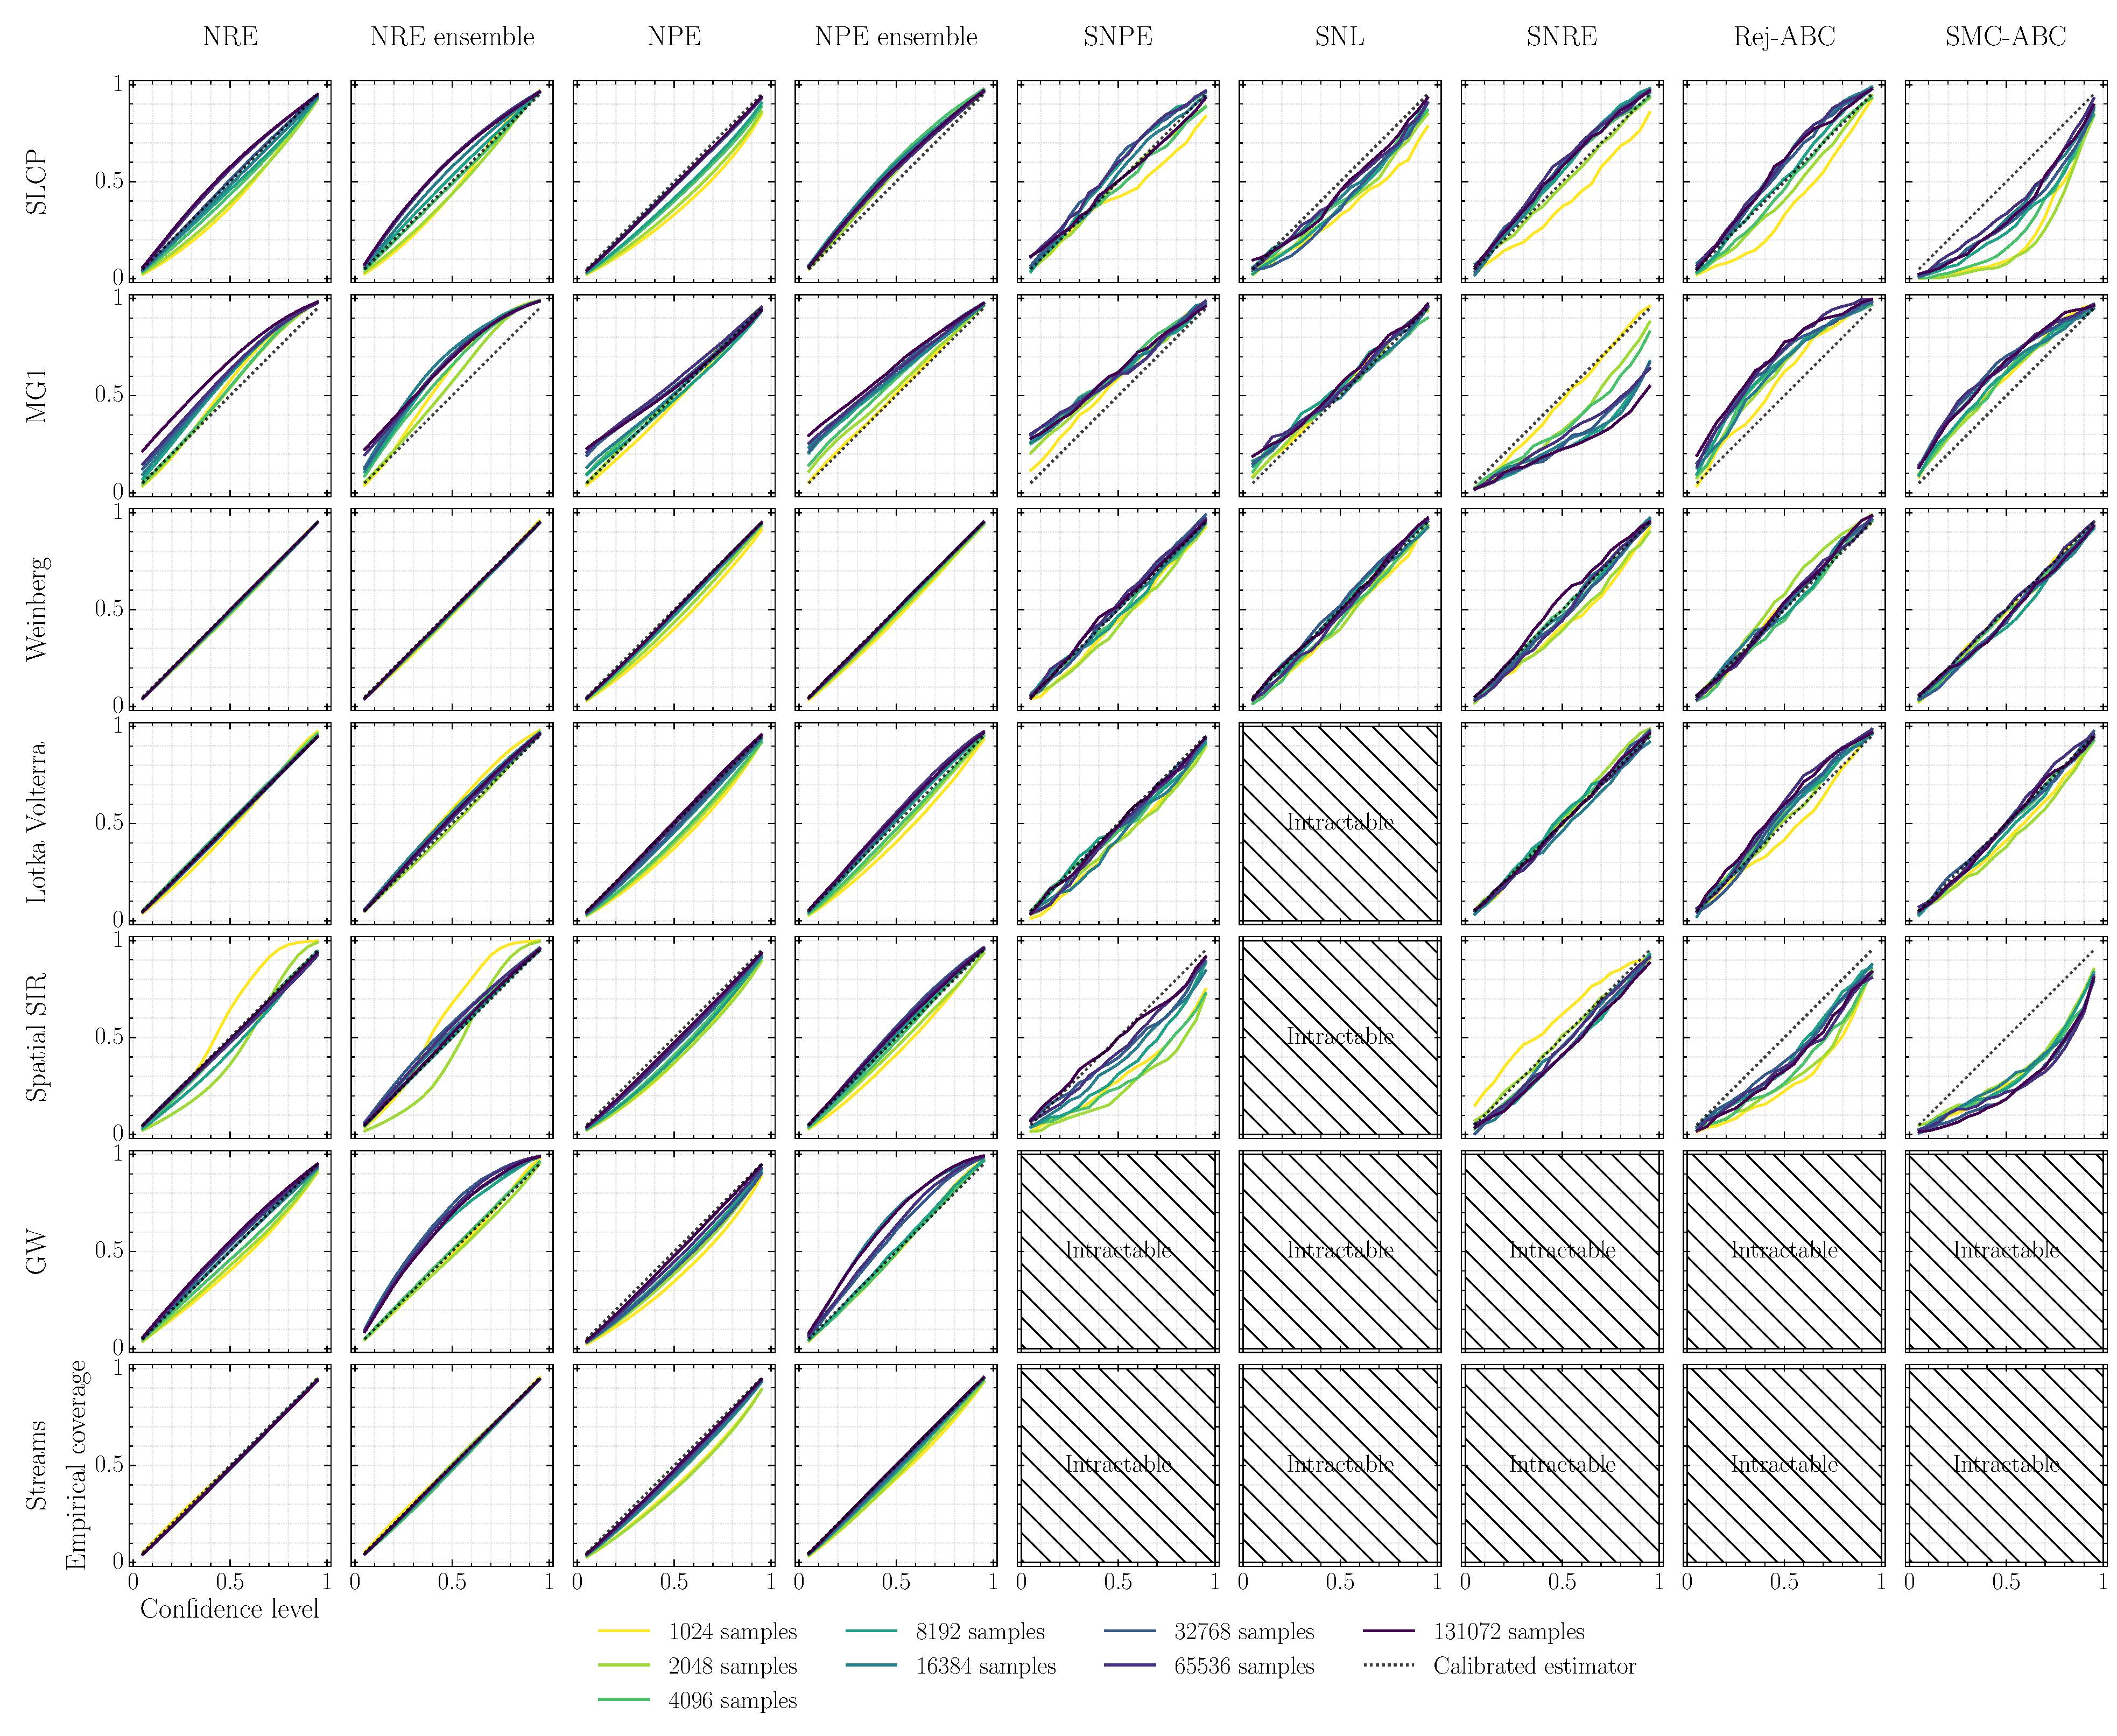
\includegraphics[width=\textwidth]{figures/coverage_multi.pdf}
    \caption{Evolution of the coverage w.r.t simulation budget. A perfectly calibrated posterior has an empirical coverage probability equal to the nominal coverage probability and produces a diagonal line. Conservative estimators on the other hand produce curves above the diagonal and overconfident models underneath. All algorithms can lead to non-conservative estimators, this pathology tends to be accentuated for small simulation budgets and non-amortized methods.
    Finally, the intractable results indicate that the computational requirements did not allow for a coverage analysis. In the case of \textsc{snl}, this was mostly due to the high dimensional observables. We did not train an embedding network as that is outside of the scope of this work. For the astronomy applications, the simulation model was simply too expensive to reasonable evaluate coverage for non-amortized methods.
    }
    \label{fig:all_coverage_levels}
\end{figure*}
\begin{figure*}[h!]
    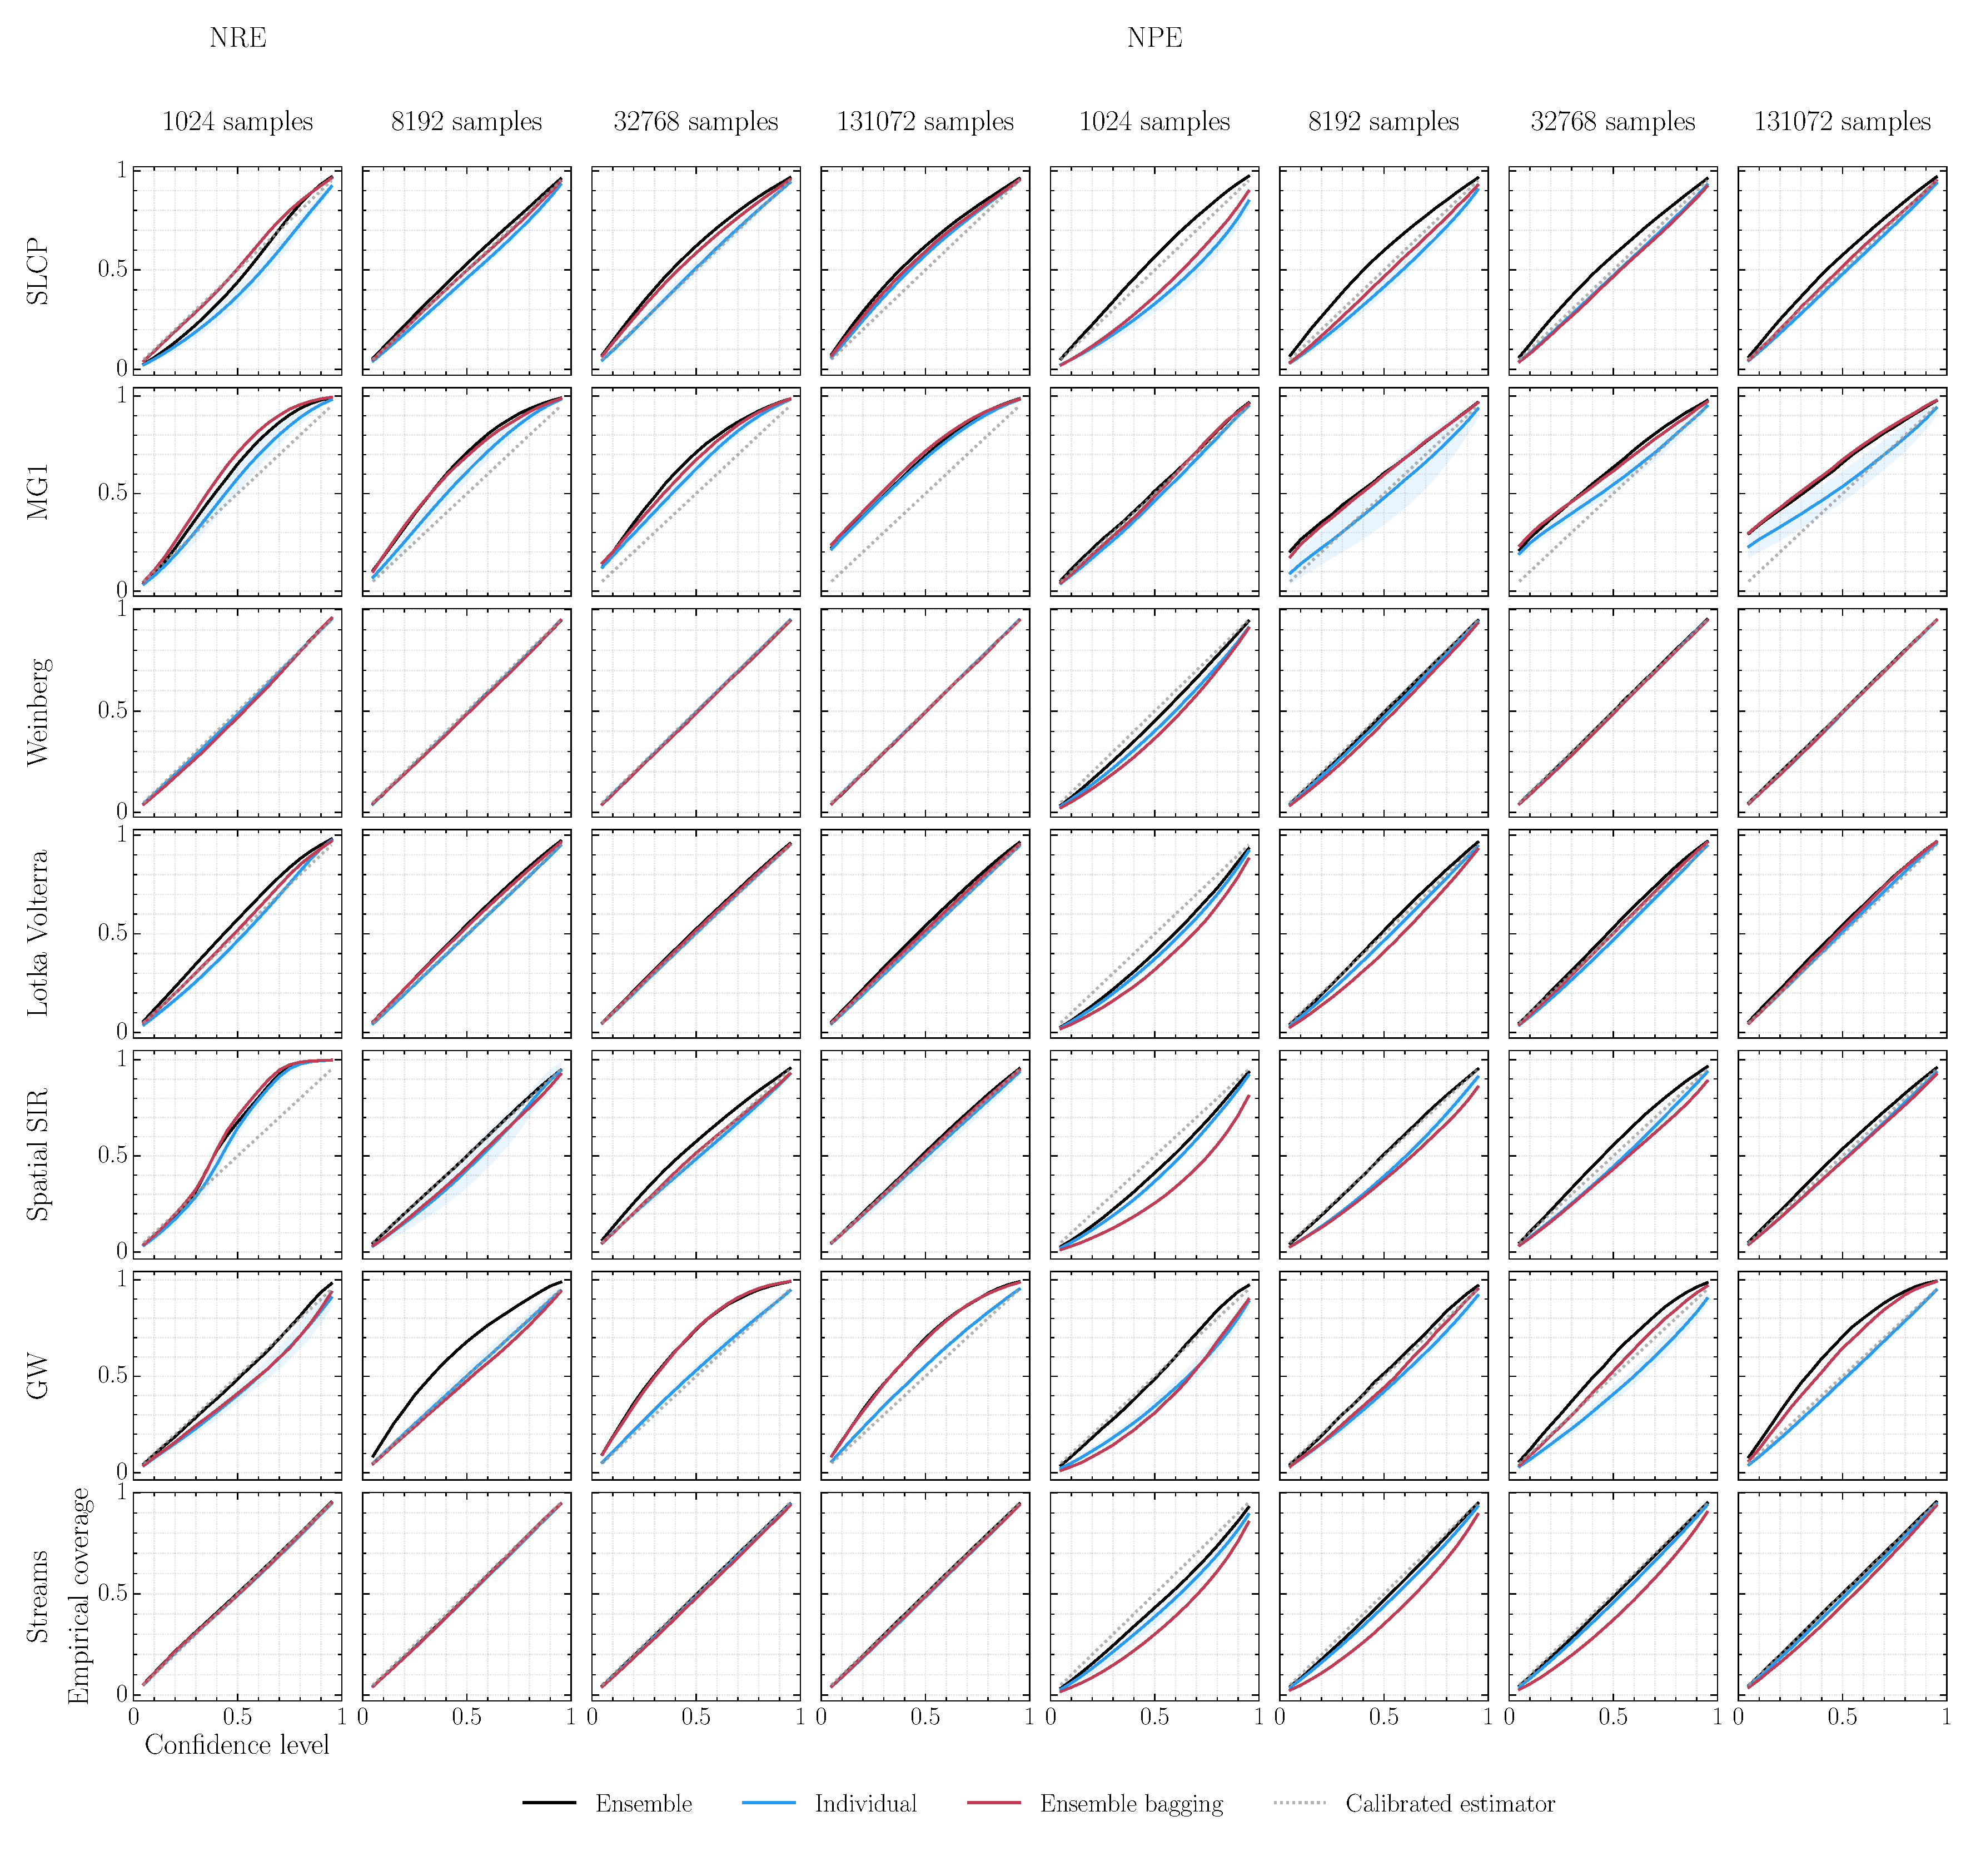
\includegraphics[width=\textwidth]{figures/coverage_multi_ensemble_with_bagging.pdf}
    \caption{Analysis of coverage between ensemble and individual models w.r.t various simulation budgets. The blue line represents the mean coverage of individual models over 5 runs, the shaded area represents its standard deviation. The black line represents the coverage of a single ensemble composed of 5 models. We observe that ensembles consistently have a higher empirical coverage probability compared to the average individual model. A similar effect is not always observed with bagging, indicated by the red line. Ensembles are only considered on amortized approached due to computational requirements inherent to non-amortized approaches.}
    \label{fig:coverage_ensemble}
\end{figure*}
Figures \ref{fig:all_coverage_levels} and \ref{fig:coverage_ensemble} highlight our main results. Through these plots we can directly assess the \emph{conservativeness} at a given confidence level and simulation budget. The figures should be interpreted as follows: a \emph{perfectly calibrated} posterior has an empirical coverage probability equal to the nominal coverage probability and therefore the known confidence level. Plotting this relation produces a diagonal line. Conservative estimators on the other hand produce curves above the diagonal and overconfident models underneath.
The plots highlight an unsettling observation: {\bfseries all} benchmarked approaches produce non-conservative posterior approximations. In general, this pathology is especially prominent in non-amortized approaches with a small simulation budget. A regime they have been specifically designed for. However, a large simulation budget does not guarantee conservativeness either.

In sequential approaches, this behaviour can be explained by the alternating exploitation and simulation phase. One potential failure mode
is that a non-conservative posterior approximation at a previous iteration forces the next simulation phase to not produce observables
that should in fact be associated with a higher posterior density, causing the estimator to be more non-conservative at each iteration.
Extreme cases were observed in the form of posterior approximations that have density \emph{outside} of the support of the prior.

Despite the fact that all \textsc{abc} approaches use a sufficient summary statistic (the identity function), our results demonstrate that this alone is no guarantee for conservative posterior approximations. In fact,
using a sufficient summary statistic with $\epsilon > 0$ does not always, as demonstrated, correspond to conservative approximations.
In such cases, \textsc{abc} accepts
samples with larger distances, permitting the procedure to shift the mass of the approximated posterior elsewhere. In addition, a limited number of posterior samples can negatively affect the quality of the credible regions, e.g., when approximating the posterior density function with kernel density estimation.
Both cases cause the observed behaviour. Scientific applications should therefore be cautious when applying \textsc{abc}. Even though a handcrafted, albeit sufficient, summary statistic provides some insight into the approximated posterior, there are no guarantees that \textsc{abc} approximations are conservative whenever $\epsilon > 0$.

In Figure \ref{fig:coverage_ensemble} we observe that the empirical coverage probability of ensemble models is consistently larger than the empirical coverage probability of the expected individual posterior estimator. Current applications of simulation-based inference can therefore rely on ensembling to build increasingly conservative posterior estimators. However, the ensemble model can still be non-conservative. We hypothesize that the increase in coverage is linked to the added uncertainty captured by the ensemble model, leading to inflated credible regions. In fact, individual estimators only captures aleatoric uncertainty, i.e., uncertainty that is linked to stochasticity of the data generation procedure, while an ensemble is expected to capture \emph{part} of the epistemic uncertainty as well, i.e., uncertainty issued by the lack of knowledge. Surprisingly, we find that ensembles built using bagging do not always produce higher coverage than individual models while they should also capture part of the epistemic uncertainty. Although a deeper understanding of this effect would be required, this behaviour could be explained by the fact that bagging reduces the effective dataset size used to train each member of the ensemble. As shown in Appendix \ref{sec:additional_results}, a positive effect with respect to ensemble size is observed.

Not evident from Figures \ref{fig:all_coverage_levels} and \ref{fig:coverage_ensemble}
are the computational consequences of a necessary coverage analysis on non-amortized methods.
Although the figures mention a certain simulation budget, the \emph{total} number of simulations for non-amortized methods should be multiplied by the number of approximated posteriors (300) to estimate coverage, highlighting the simulation cost associated with diagnosing non-amortized approaches.
This observation issue is not limited to coverage. Simulation-Based Calibration (\textsc{sbc}) \citep{sbc} relies on samples of arbitrary posterior approximations.
Diagnosing non-amortized estimators with \textsc{sbc} therefore
requires a similar approach as we have taken in our coverage analyses.
In fact, \citet{lueckmann2021benchmarking} also mention that \textsc{sbc} is computationally prohibitive for non-amortized (sequential) approaches and therefore restrain from evaluating it.

Our results illustrate a clear distinction between the amortized and non-amortized paradigms. Amortized methods do not require retraining or new simulations to determine the empirical coverage probability of a posterior estimator, while non-amortized methods do.
Moreover, a coverage analysis of non-amortized approaches only measures the quality of the training procedure. In contrast to amortized approaches, where the posterior estimator is diagnosed.
This has severe
implications on the applicability of non-amortized methods, because their reliability cannot be practically determined. In addition, non-amortized approaches have to repeat the approximation procedure whenever architectural or hyperparameter changes are made, while amortized methods reuse previously simulated datasets. In particular, sequential methods cannot do this as new simulations depend on the posterior approximation at a previous state. This is often overlooked in studies on simulation efficiency and raises questions about whether sequential approaches should still be considered simulation efficient over their amortized counterparts. Especially because our results indicate that for a given simulation budget, amortized approaches produce trustworthier posterior approximations in expectation.

All of the above leads us to conclude that \emph{currently}, amortization should be favoured over non-amortized approaches because they are tedious to diagnose. Remarkably, our results suggest that even for small simulation budgets amortized methods do in fact, on average, produce more conservative posterior estimators compared to non-amortized methods.
A striking result, given that sequential methods dedicate the available simulation budget to accurately approximate a single posterior. No clear distinction between \textsc{nre} and \textsc{npe} was observed. Although interestingly, ensembling leads to significant improvements with respect to coverage.

\section{Discussion}
\label{sec:discussion}
%This work establishes that \textsc{(s)npe}, \textsc{(s)nre}, \textsc{snl} and various forms of \textsc{abc} can produce non-conservative posterior approximations. Performing a coverage-like diagnostic is therefore necessary before applying the learned posterior estimator.
Assessing the \emph{correctness} of posterior approximations is not restricted to simulation-based inference specifically, the question recurs in all of approximate Bayesian inference.
In particular, the \textsc{mcmc} literature deals with this exact same problem in the form of determining whether a set of Markov chain samples have \emph{converged} to the target distribution \citep{lin2014integrated,hogg2018data}.
Although empirical diagnostic tools exist \citep{geweke1991evaluating,gelman1992inference,raftery1991many,dixit2017mcmc},
there is as no clear solution to determine covergence with absolute certainty \citep{dixit2018developments,roy2020convergence}, even though the evaluation of the likelihood model is tractable.
Nevertheless, this has not prevented practitioners from applying \textsc{mcmc}, especially when considering the theoretical guarantees that come with the samplers. For this reason, we are of the opinion that theoretical and methodological advances in simulation-based inference (beyond global optima) will improve the reliability of simulation-based inference and promote its applibability in the sciences.

Recently, \citet{dalmasso2021likelihood} have explored this direction in the frequentist setting by introducing an algorithm for the construction of confidence intervals that are guaranteed to have perfect coverage in the infinite sample setting regardless of the quality of the statistic used. In the finite sample setting, they provide a theoretical bound on the approximation error.
However, this bound is an absolute value and does not ensure conservativeness for a given simulation budget.

Our results show that ensembling produce increasingly conservative posteriors. Ensembles and model averaging in general, including the field of Bayesian deep learning, constitute a promising research direction. A theoretical understanding of these frameworks in the context of simulation-based inference would further strengthen their applicability.

Finally, despite that the benchmarked algorithms recover the true posterior under specific optimal conditions, it is generally not possible to know whether those conditions are satisfied in practice.
The study of objective functions that force posterior estimators to be conservative, regardless of whether their fitting criteria have been globally minimized, is therefore worth exploring. However, it is not clear as of yet on how to define and encode conservativeness in objective functions. Nevertheless, such objective functions would establish formal guarantees and strengthen the reliability of posterior estimators regardless of the available simulation budget.

\subsubsection*{Acknowledgements}
Antoine Wehenkel, Arnaud Delaunoy, and Joeri Hermans would like to thank the National Fund for Scientific Research (F.R.S.-FNRS) for their scholarships.
Gilles Louppe is recipient of the ULiège - NRB Chair on Big Data and is thankful for the support of the NRB. Computational resources have been provided by the Consortium des Équipements de Calcul Intensif (CÉCI), funded by the National Fund for Scientific Research (F.R.S.-FNRS) under Grant No. 2.5020.11 and by the Walloon Region.

\bibliographystyle{plainnat}
\bibliography{main}

% Appendix
\clearpage
\newpage
\appendix

\onecolumn
\section*{Appendix}
\label{appendix}

\section{Expected simulation times}
\label{appendix:simulation_times}
\begin{table}[h!]
    \centering
    \begin{tabular}{lllllll}
        \toprule
        SLCP & M/G/1 & Weinberg & Lotka-V. & Spatial SIR & GW & Streams \\
        \midrule
        $0.22\pm 0.002$ & $0.20\pm 0.002$ & $0.20\pm 0.002$ & $19.08\pm 0.964$ & $9.18\pm 0.280$ & $545.13\pm 23.631$ & $39,369 \pm 584.43$ \\
        \bottomrule
    \end{tabular}
    \caption{Expected simulation time to produce 1000 simulations for all benchmark problems on a single CPU core. The expected time and standard deviation is reported in seconds.}
    \label{tab:simulation_times}
\end{table}

\section{Architectures \& hyperparameters}
\label{appendix:hyperparameters}
In this section we describe the neural architectures and hyperparameters associated with our experiments. Our descriptions are complemented with the actual number of coverage evaluations. As evident from the tables describing both amortized and non-amortized approaches, the number of coverage evaluations for amortized approaches is substantially larger. It should be noted that, a coverage analysis consisting of 300 posteriors of the non-amortized approaches took \emph{months} on these relatively simple problems. While for the amortized methods, a coverage analysis of 100,000 samples was a matter of hours to a few days depending on the dimensionality of $\vtheta$.

\subsection{Amortized}
\subsubsection{Neural Posterior Estimation}
The MLP embeddings are 3 layer MLP's with 64 hidden units and a final latent space of 10, which is fed to the normalizing flow.
The CNN architecture in the Gravitational Waves benchmark consists of a 13-layer deep convolutional head of 1D convolutions with a dilation factor of $2^d$. Where $d$ corresponds to the depth of the convolutional head. The SELU \citep{selu} function is used as an activation function.
\begin{table}[h!]
    \centering
    \begin{tabular}{llllllll}
        \toprule
        & SLCP & M/G/1 & Weinberg & Lotka-V. & Spatial SIR & GW & Streams \\
        \midrule
        \emph{Embedding} & MLP & MLP & MLP & MLP & MLP & CNN & MLP \\
        \emph{Batch-size} & 128 & 128 & 128 & 128 & 128 & 64 & 128 \\
        \emph{Coverage samples individual} & 100,000 & 5,000 & 100,000 & 100,000 & 100,000 & 10,000 & 100,000 \\
        \emph{Coverage samples ensemble} & 20,000 & 5,000 & 20,000 & 20,000 & 20,000 & 5,000 & 20,000 \\
        \emph{Epochs} & 100 & 100 & 100 & 100 & 100 & 100 & 100 \\
        \emph{Model} & NSF & NSF & NSF & NSF & NSF & NSF & NSF \\
        \emph{Transforms} & 3 & 3 & 1 & 3 & 3 & 3 & 3 \\
        \emph{Learning-rate} & 0.001 & 0.001 & 0.001 & 0.001 & 0.001 & 0.001 & 0.001 \\
        \bottomrule
    \end{tabular}
    \caption{Architectures and hyperparameters associated with Neural Posterior Estimation.}
    \label{tab:npe_hyperparameters}
\end{table}

\subsubsection{Neural Ratio Estimation}
Our experiments use the \textsc{adamw} \citep{adam,adamw} optimizer. Accross all benchmarks, the MLP architectures constitute of 3 hidden layers with 128 units and SELU \citep{selu} activations. The Gravitational Waves benchmark uses the same convolutional architecture as in \textsc{npe}. The resulting embedding is flattened and fed to a MLP in which the dependence on the target parameter $\vtheta$ is added. As before, the MLP consists of 3 hidden layers with 128 units.
\begin{table}[h!]
    \centering
    \begin{tabular}{llllllll}
        \toprule
        & SLCP & M/G/1 & Weinberg & Lotka-V. & Spatial SIR & GW & Streams \\
        \midrule
        \emph{Architecture} & MLP & MLP & MLP & MLP & MLP & CNN & MLP \\
        \emph{Batch-size} & 128 & 128 & 128 & 128 & 128 & 64 & 128 \\
        \emph{Coverage samples individual} & 100,000 & 100,000 & 100,000 & 100,000 & 100,000 & 10,000 & 100,000 \\
        \emph{Coverage samples ensemble} & 20,000 & 20,000 & 20,000 & 20,000 & 20,000 & 10,000 & 20,000 \\
        \emph{Epochs} & 100 & 100 & 100 & 100 & 100 & 100 & 100 \\
        \emph{Learning-rate} & 0.001 & 0.001 & 0.001 & 0.001 & 0.001 & 0.001 & 0.001 \\
        \bottomrule
    \end{tabular}
    \caption{Architectures and hyperparameters associated with Neural Ratio Estimation.}
    \label{tab:npe_hyperparameters}
\end{table}

\subsection{Non-amortized}
All our implementations of non-amortized approaches rely on the reference implementation in \texttt{sbi} \citep{sbi}. We use the recommended defaults unless stated otherwise. Whenever available, the same MLP embedding network is used. It consists of 3 hidden layers with 64 units and SELU \citep{selu} activations. The latent space has a dimensionality of 10 features. For all sequential methods, we use 10 rounds to iteratively improve the posterior approximation.
\subsubsection{SNPE}
Our evaluations with \textsc{snpe} specifically use the \textsc{snpe-c} \citep{greenberg2019automatic} variant, as suggested by \texttt{sbi} \citep{sbi}.
To minimize inconsistencies between experiments, we use the defaults suggested by the \texttt{sbi} authors unless states otherwise. Specific changes are highlighted in Table \ref{tab:snpe_hyperparameters}.

\begin{table}[h!]
    \centering
    \begin{tabular}{llllllll}
        \toprule
        & SLCP & M/G/1 & Weinberg & Lotka-V. & Spatial SIR & GW & Streams \\
        \midrule
        \emph{Batch-size} & 128 & 128 & 128 & 128 & 32 & Intractable & Intractable \\
        \emph{Coverage samples} & 300 & 300 & 300 & 300 & 300 & Intractable & Intractable \\
        \emph{Embedding} & MLP & MLP & MLP & MLP & MLP & Intractable & Intractable \\
        \emph{Epochs} & 100 & 100 & 100 & 100 & 100 & Intractable & Intractable \\
        \emph{Features} & 64 & 64 & 64 & 64 & 64 & Intractable & Intractable \\
        \emph{Model} & NSF & NSF & NSF & NSF & NSF & Intractable & Intractable \\
        \emph{Transforms} & 3 & 3 & 1 & 3 & 3 & Intractable & Intractable \\
        \emph{Rounds} & 10 & 10 & 10 & 10 & 10 & Intractable & Intractable \\
        \emph{Learning-rate} & 0.001 & 0.001 & 0.001 & 0.001 & 0.001 & Intractable & Intractable \\
        \bottomrule
    \end{tabular}
    \caption{Architectures and hyperparameters associated with Sequential Neural Posterior Estimation.}
    \label{tab:snpe_hyperparameters}
\end{table}

\subsubsection{SNL}
In contrast to other sequential methods, our evaluations with \textsc{snl} \citep{papamakarios2019sequential} add two additional intractable benchmarks. At the root of this issue lies the dimensionality of the observable. In both cases, the dimensionality of observables caused memory issues in \textsc{snl}. In addition, training a seperate embedding model (that requires additional simulations) is outside of the scope of this work. For this reason, we consider the Lotka-Volterra en Spatial SIR benchmark to be intractable.

\begin{table}[h!]
    \centering
    \begin{tabular}{llllllll}
        \toprule
        & SLCP & M/G/1 & Weinberg & Lotka-V. & Spatial SIR & GW & Streams \\
        \midrule
        \emph{Batch-size} & 128 & 128 & 128 & Intractable & Intractable & Intractable & Intractable \\
        \emph{Coverage samples} & 300 & 300 & 300 & Intractable & Intractable & Intractable & Intractable \\
        \emph{Epochs} & 100 & 100 & 100 & Intractable & Intractable & Intractable & Intractable \\
        \emph{Features} & 64 & 64 & 64 & Intractable & Intractable & Intractable & Intractable \\
        \emph{Model} & NSF & NSF & NSF & Intractable & Intractable & Intractable & Intractable \\
        \emph{Transforms} & 3 & 3 & 1 & Intractable & Intractable & Intractable & Intractable \\
        \emph{Rounds} & 10 & 10 & 10 & Intractable & Intractable & Intractable & Intractable \\
        \emph{Learning-rate} & 0.001 & 0.001 & 0.001 & Intractable & Intractable & Intractable & Intractable \\
        \bottomrule
    \end{tabular}
    \caption{Architectures and hyperparameters associated with Sequential Neural Likelihood.}
    \label{tab:snl_hyperparameters}
\end{table}

\newpage
\subsubsection{SNRE}
\begin{table}[h!]
    \centering
    \begin{tabular}{llllllll}
        \toprule
        & SLCP & M/G/1 & Weinberg & Lotka-V. & Spatial SIR & GW & Streams \\
        \midrule
        \emph{Architecture} & MLP & MLP & MLP & MLP & MLP & Intractable & Intractable \\
        \emph{Batch-size} & 128 & 128 & 128 & 128 & 128 & Intractable & Intractable \\
        \emph{Coverage samples} & 300 & 300 & 300 & 300 & 300 & Intractable & Intractable \\
        \emph{Epochs} & 100 & 100 & 100 & 100 & 100 & Intractable & Intractable \\
        \emph{Features} & 64 & 64 & 64 & 64 & 64 & Intractable & Intractable \\
        \emph{Rounds} & 10 & 10 & 10 & 10 & 10 & Intractable & Intractable \\
        \emph{Learning-rate} & 0.001 & 0.001 & 0.001 & 0.001 & 0.001 & Intractable & Intractable \\
        \bottomrule
    \end{tabular}
    \caption{Architectures and hyperparameters associated with Sequential Neural Ratio Estimation.}
    \label{tab:snre_hyperparameters}
\end{table}

\subsubsection{Approximate Bayesian Computation}
Our \textsc{abc} implementation relies on the \texttt{MCABC} and \texttt{SMCABC} classes in the \texttt{sbi} \citep{sbi} package.
The specific settings from Rejection \textsc{abc} and \textsc{smc-abc} are described in Tables \ref{tab:abc_hyperparameters} and \ref{tab:smcabc_hyperparameters} respectively.
The quantile specifically refers to the proportion of closest samples that were kept in the final posterior. Because our specific implementation our coverage requires the ability to describe the posterior density function, we relied on Kernel Density Estimation to estimate the posterior density from the accepted samples.
\begin{table}[h!]
    \centering
    \begin{tabular}{llllllll}
        \toprule
        & SLCP & M/G/1 & Weinberg & Lotka-V. & Spatial SIR & GW & Streams \\
        \midrule
        \emph{Coverage samples} & 300 & 300 & 300 & 300 & 300 & Intractable & Intractable \\
        \emph{Quantile} & 0.01 & 0.01 & 0.01 & 0.01 & 0.01 & Intractable & Intractable \\
        \bottomrule
    \end{tabular}
    \caption{Hyperparameters associated with Rejection Approximate Bayesian Computation.}
    \label{tab:abc_hyperparameters}
\end{table}
\begin{table}[h!]
    \centering
    \begin{tabular}{llllllll}
        \toprule
        & SLCP & M/G/1 & Weinberg & Lotka-V. & Spatial SIR & GW & Streams \\
        \midrule
        \emph{Coverage samples} & 300 & 300 & 300 & 300 & 300 & Intractable & Intractable \\
        \emph{$\epsilon$ decay} & 0.5 & 0.5 & 0.5 & 0.5 & 0.5 & Intractable & Intractable \\
        \emph{Quantile} & 0.01 & 0.01 & 0.01 & 0.01 & 0.01 & Intractable & Intractable \\
        \bottomrule
    \end{tabular}
    \caption{Hyperparameters associated with Sequential Monte Carlo Approximate Bayesian Computation.}
    \label{tab:smcabc_hyperparameters}
\end{table}

%\section{Benchmarks}
%\label{appendix:benchmarks}
%\subsection{SLCP}
%\subsection{M/G/1}
%\subsection{Weinberg}
%\subsection{Lotka Volterra}
%\subsection{Spatial SIR}
%\subsection{Gravitational Waves}
%\subsection{Stellar Streams}

\clearpage
\newpage
\section{Additional results}
\label{sec:additional_results}
\begin{figure}[h!]
    \centering
    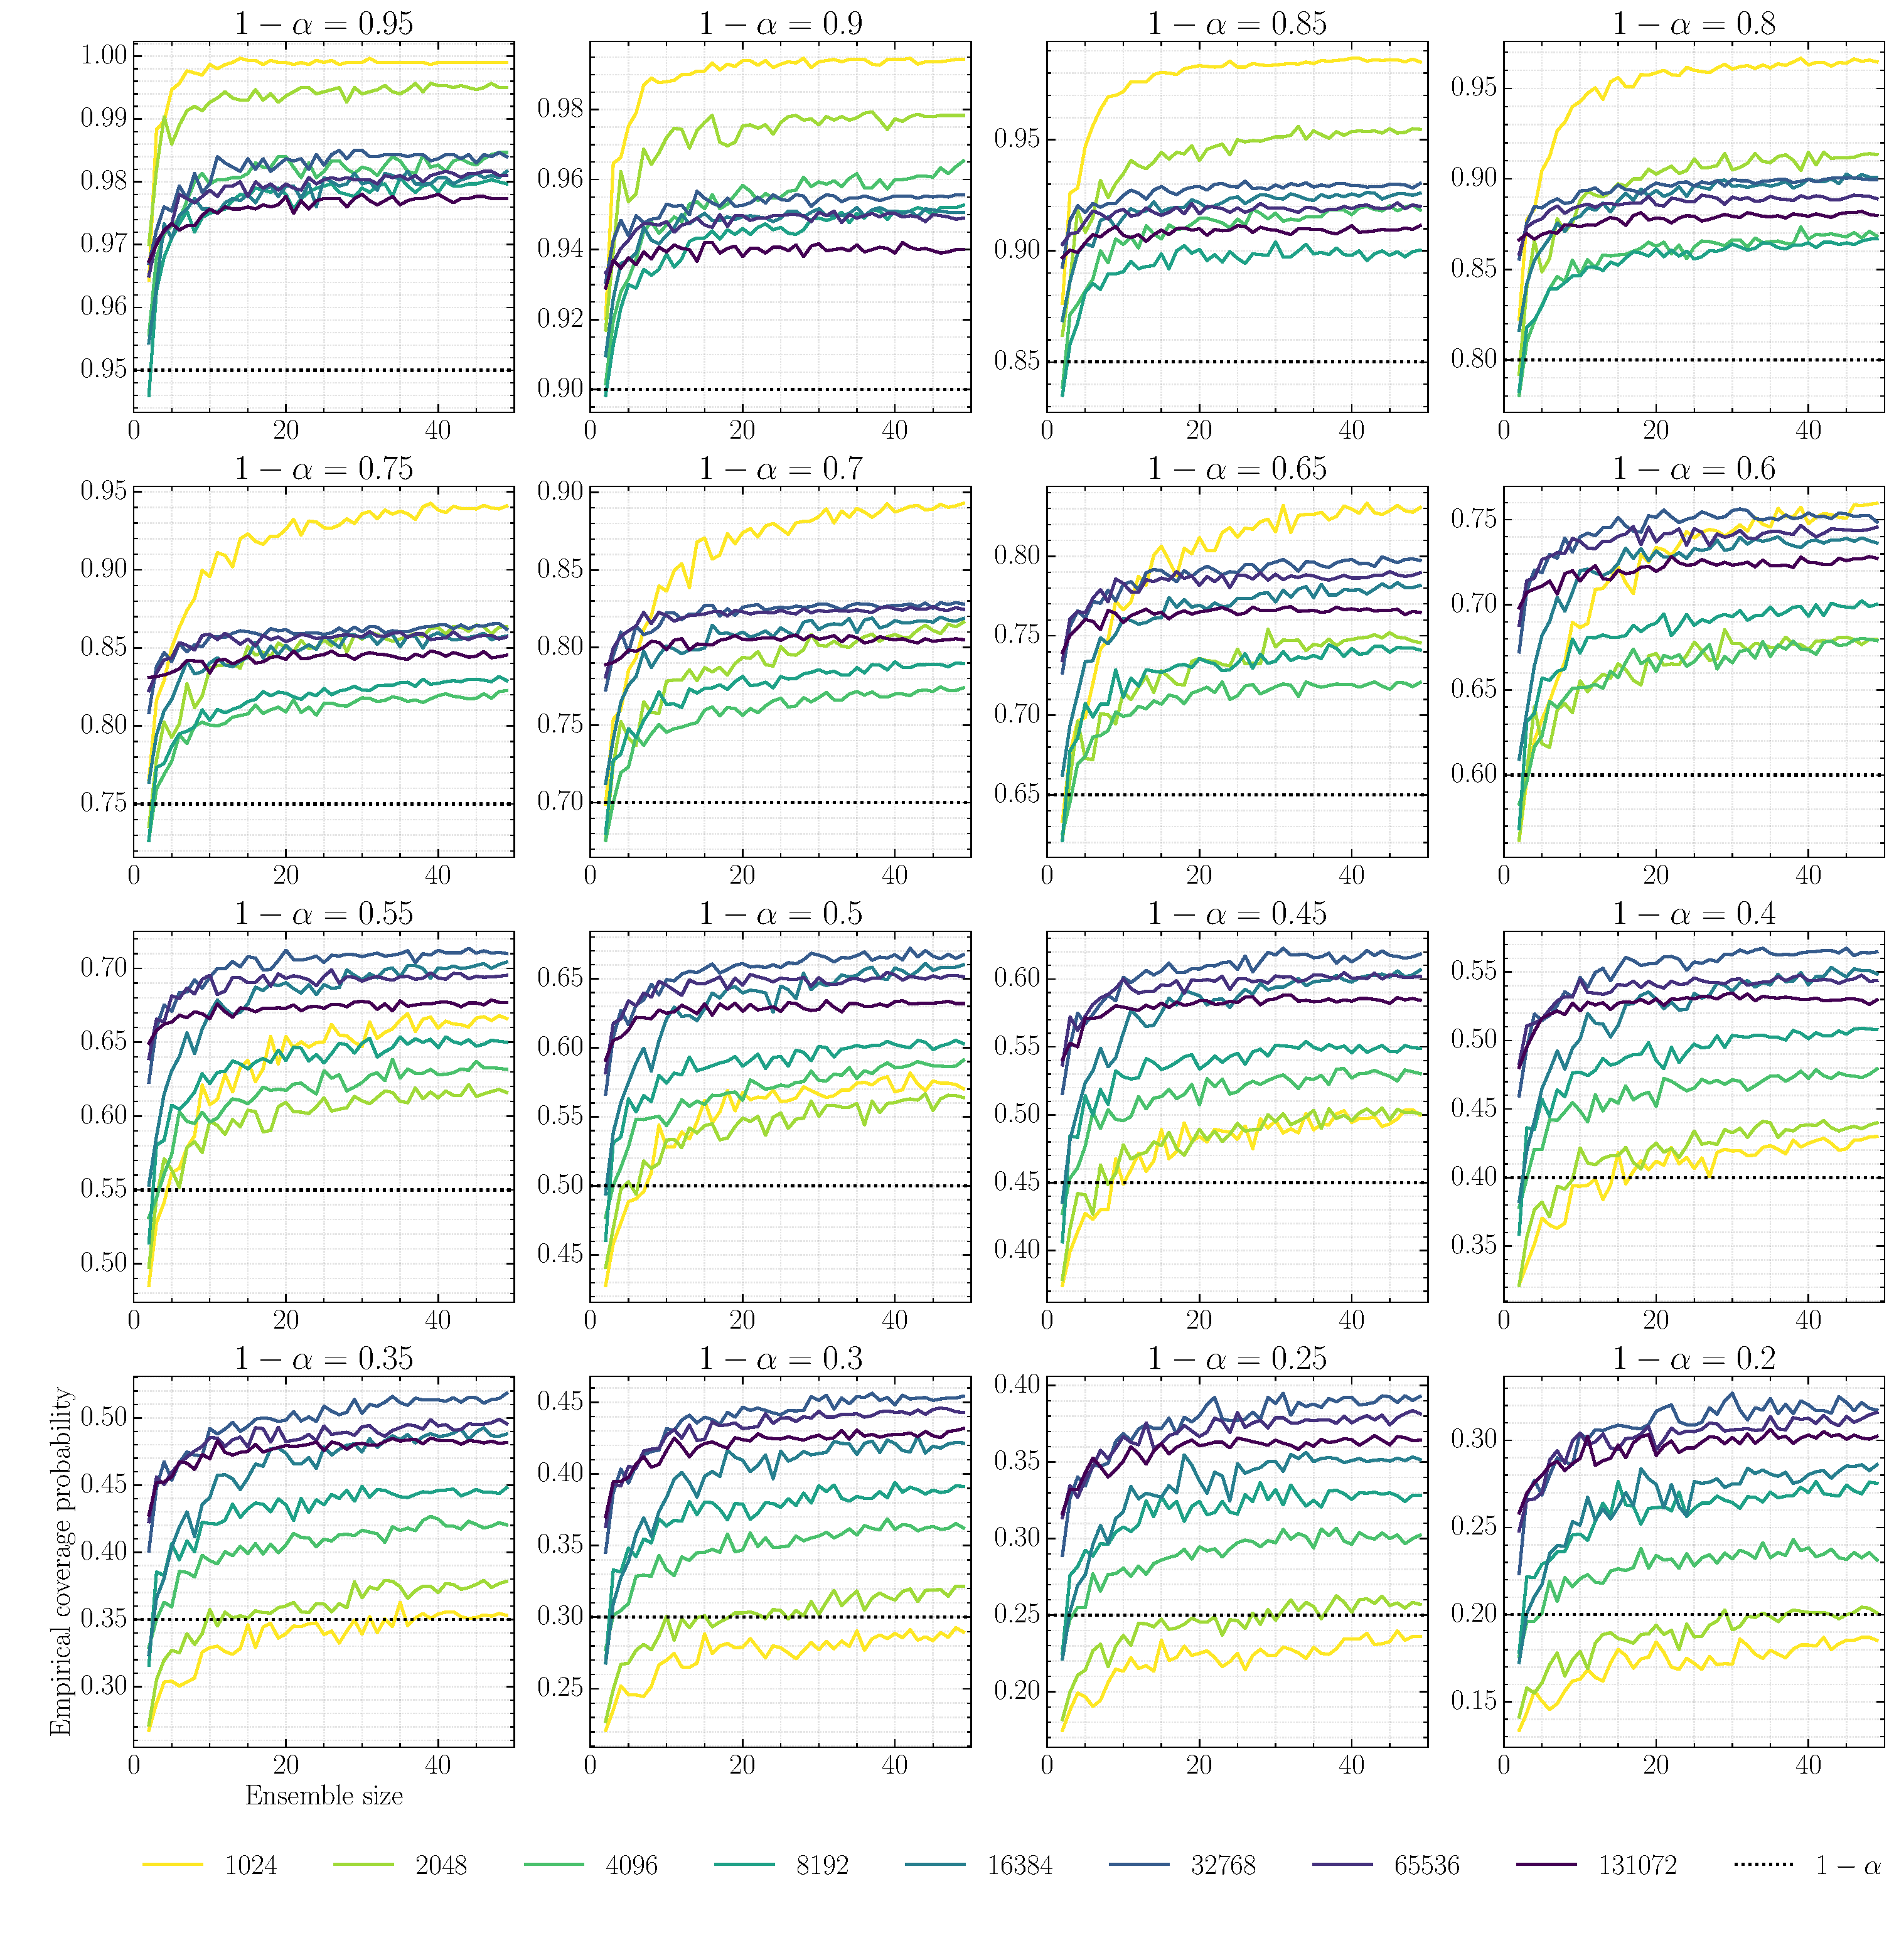
\includegraphics[width=\linewidth]{figures/coverage_ensemble_size}
    \caption{Evolution of the empirical coverage probability with respect to ensemble size for various confidence levels. The results are obtained by training 100 ratio estimators (\textsc{nre}) on the \textsc{slcp} benchmark. A positive effect is observed in terms of empirical coverage probability and ensemble size, i.e., a larger ensemble size correlates with a larger empirical coverage probability. This is not unsurprising, because a larger ensemble is expected to capture more of the uncertainty that stems from the training procedure.}
    \label{fig:coverage_ensemble_size}
\end{figure}

\end{document}
